%Template and commentary by Michael Rouleau: https://github.com/mikerouleau/ME4842.git
%Text primarily from Dr. Stutts' Systems Laboratory Manual /ref{Stutts}
%Last Updated: Feb 17, 2019

%----This template includes equation captions and numbering BELOW the equation, as required by Blaine Allen----%

\documentclass[11pt,letter]{report}
\usepackage[margin=1in]{geometry} %make margins 1"
\usepackage[justification=centering, format=plain, font=it, margin=1in]{caption} %all captions centered and made italics by default
\usepackage{amsmath, amssymb} %advanced math extensions
\usepackage{graphicx} %enhanced graphics handling/management
\usepackage{float} %create floating containers
\usepackage{aliascnt} %alias counters as needed


%for the commentary section only
\usepackage[british]{babel}
\usepackage{hyperref}
\usepackage{xcolor}
\definecolor{lightgray}{gray}{0.93}
\usepackage{listings} %For code in appendix
\lstset{language = [LaTeX]TeX,     breaklines=true,
	numbers=left, backgroundcolor=\color{lightgray}}

%make equations floating objects and alias counter - needed for formatting requirements
\newaliascnt{eqfloat}{equation} %make the counter alias eqfloat
\newfloat{eqfloat}{!htb}{eqflts} %make the float container for equations
\floatname{eqfloat}{Equation} %change name so captions read "Equation" X:

%nontraditional usage of author to meet formatting requirements
\title{\Huge{Systems Lab \LaTeX\ Template Commentary}}
\author{Section \#, Group \#: \\
	Group Member 1 \footnote{Missouri University of Science and Technology, Rolla, Missouri 65409} 
	\quad Group Member 2\footnotemark[1]
	\quad Group Member 3\footnotemark[1]
	\quad Group Member 4\footnotemark[1] 
	\\ GTA: Best GTA Ever\footnotemark[1] \\ \\ 
	Prepared By: \\ Michael Rouleau\footnote{Georgia Institute of Technology, Atlanta, Georgia 80813}
}
\date{\today}

\begin{document}
	\maketitle
	
	\chapter{Using \LaTeX{}} \label{chap:usinglatex}
	\section{About \LaTeX{}}
	\LaTeX{}, pronounced "Lah-tech" or "Lay-tech" \cite{Lamport}, is an advanced document preparation system popular in the scientific world and academia. Instead of organizing a document visually like a WYSIWYG (what you see is what you get) package (e.g. Microsoft Word), \LaTeX{} has a logical structure that focuses on content rather than formatting decisions. This means that if you decide that all of your fractions of the form $\tfrac{x}{y}$ require a little extra size, as in $\dfrac{x}{y}$, the entire document can be reformatted with just a line or two of code. Similarly, it is possible to compile a list of sources that were used during research, then automatically list and number only those which were cited in the manuscript. Citations auto-update. Updating figures is a breeze. Complex mathematical notations are just a few keystrokes away. For long scientific documents, \LaTeX{} is the cat's meow.
	
	\section{Installation} \label{sect:install}
	To start editing a \LaTeX{} document on a Missouri S\&T Computer, simply log on to AppsAnywhere and start the program ``Texmaker."
	
	For personal computers, Texmaker is freely available from \url{http://www.xm1math.net/texmaker/}; its dependency, MiKTeX, is available from \url{https://miktex.org/}. Installing MiKTex before Texmaker is highly recommended. Detailed installation instructions are available on each package's respective website. It is possible to run a portable installation of the above from a USB drive.
	
	Online editors are also available  - Overleaf \cite{Overleaf}, for example, is a free collaborative editor somewhat similar to Google Docs.
	
	\section{Basics} \label{sect:basics}
	\subsection{Syntax}
	\LaTeX{} code is typed into a plain-text file called an ``input" or ``source" file that contains markup which tells the compiler how to display content. In general, the following reserved characters demarcate normal text from commands or other special functions:
	
	\begin{center}		
		\# \$ \% \^{} \& \_ \{ \} \~{} \textbackslash{}.
	\end{center}
	
	\newpage
	It is still possible to use these symbols, but they typically require a backslash prefix or other special notation.
	
	\begin{center}		
		\verb|\# \$ \% \^{} \& \_ \{ \} \~{} \textbackslash{}|
	\end{center}
	
	Commands also usually require a backslash prefix. For example, the command
	\verb|\textbf{text}| turns \textbf{text} bold. Most commands can be nested; \verb|\textbf{\textit{Italics and Bold!}}| turns text both \textit{\textbf{Italics and Bold!}}
	
	Likewise, backslashes are required to begin an environment. Environments act similar to commands but are usually applied to multiple lines or used for more complex operations. For example, the following code would insert a picture file named ``joeminer" located in the directory where the \LaTeX{} file is saved.
	\begin{lstlisting}[numbers=left,xleftmargin=5mm]
\begin{figure}
	\includegraphics{joeminer}
\end{figure}
	\end{lstlisting}	
	
	Many commands and environments are packaged with standard \LaTeX{} distributions, but more customization is available by loading external packages. One of the most popular packages, \nobreakdash graphicx, allows users to load and manipulate figures, as we did with the joeminer figure above.
	
	Coding comments can be added with the \% symbol. Following a percent symbol, the compiler will ignore the remainder of the current line and any whitespace at the beginning of the following line. This can be useful for adding notes that should not be included in the final document.
	
	\section{Structure}\label{sec:structure}
	The minimum structure of a \LaTeX{} document is best illustrated with the following Hello World example. Feel free to follow along in Texmaker.
	\begin{lstlisting}[numbers=left,xleftmargin=5mm]
\documentclass{article}
\begin{document}
	Hello World!
\end{document}
	\end{lstlisting}
	
	
	Breaking down each line, we first have an initial declaration of which class the document is - this sets basic definitions for formatting. In this example, we're using the article class, which is a common starting point.
	
	The second line is where the document officially starts. This is where the environment called ``document" begins - all of your content will go between the \verb|\begin{document}| and \verb|\end{document}| tags. Everything before this point is traditionally called the ``Preamble." If you are including any external packages, changing global formatting, or redefining commands, do so in the Preamble.
	
	Our content, of course, only consists of ``Hello World!". This is where your entire report, book, manuscript, etc. would go.
	
	Finally, \verb|\end{document}| ends the document environment. Anything after this line is ignored.
	
	To compile your first \LaTeX{} document, save your file (without spaces in the name!) and click the ``Run" arrow in the top toolbar of Texmaker. Your new document should appear on the right side of the window. For simple documents, only one compilation is necessary. For complex documents (especially those with intricate cross-references), multiple compilation steps may be required.
	
	\section{Organization} \label{sect:org}
		
	\LaTeX{} commands for breaking up documents are intuitive. For example, paragraphs are created by placing a blank line in your code before the start of the next paragraph. Any more than 1 blank line is ignored. The command \verb|\chapter{Silver}| starts a new chapter named ``Silver" and \verb|\section{Gold}| starts a new section called ``Gold." It is left as an exercise for the reader to discover what \verb|\subsection{text}| and \verb|\subsubsection{text}| do.
	
	With each of these commands, a number or other counter is inserted by default. To create an unnumbered heading, the ``starred" version may be used. For example, a unnumbered section heading would use the command \verb|\section*{text}|. To manually adjust a counter, the command \verb|\setcounter{countername}{#}| is used.
	
	In \LaTeX{}, we can also define containers called ``floats." These containers are traditionally applied to things that cannot be broken over a page, like figures and tables; these are floats by default. To keep these items intact, \LaTeX{} moves floats around to a spot where they can be preserved. Since by definition these containers move around, it is beneficial to define a list of preferred locations to place the container. To do this, each float declaration takes a position argument. A handful of these options are listed below in Table \ref{tbl:positions} \cite{Overleaf}. Note that too many floats with the H specifier in a row may cause errors.
	
	\begin{table}[htb]
		\caption{Float Position Options}
		\label{tbl:positions}
		\centering
		\begin{tabular}{|l|l|}
			\hline
			Option & Permission                                                                                                                                                                                                                 \\ \hline
			h         & Place the float here, i.e., approximately at the same point it occurs in the source text.                      \\ \hline
			t         & Position at the top of the page.                                                                                                                                                                                           \\ \hline
			b         & Position at the bottom of the page.                                                                                                                                                                                        \\ \hline
			p         & Put on a special page for floats only.                                                                                                                                                                                     \\ \hline
			!         & Override internal parameters \textbackslash{}LaTeX\{\} uses for determining "good" float positions.                                                                                                                        \\ \hline
			H         & Places the float at precisely the location in the \textbackslash{}LaTeX\{\} code. \\ \hline
		\end{tabular}
	\end{table}
	
	Figures, tables, etc. may also be assigned a label using \verb|\label{key}|. This label isn't displayed in the compiled document, but allows for automatic cross-referencing elsewhere in the document. Referencing is covered in Section \ref{sect:ref}.
	
	\pagebreak
	\subsection*{Example}
	
	Let's modify our Hello World code to make use of several of the above features. Before compiling, make sure there is an image named ``figure1" in the same directory as your code. Most common file types are supported (jpg, png, etc).
	\begin{lstlisting}[numbers=left,xleftmargin=5mm]
\documentclass{article}
\usepackage{graphicx}
\begin{document}
	\section{A Clever Heading}
		\label{sect:Clever}
		This section has a number and a label!
	\section*{Figures}
		This section does not have a number displayed, but it has a figure on a dedicated page for floats!
		\begin{figure}[p]
			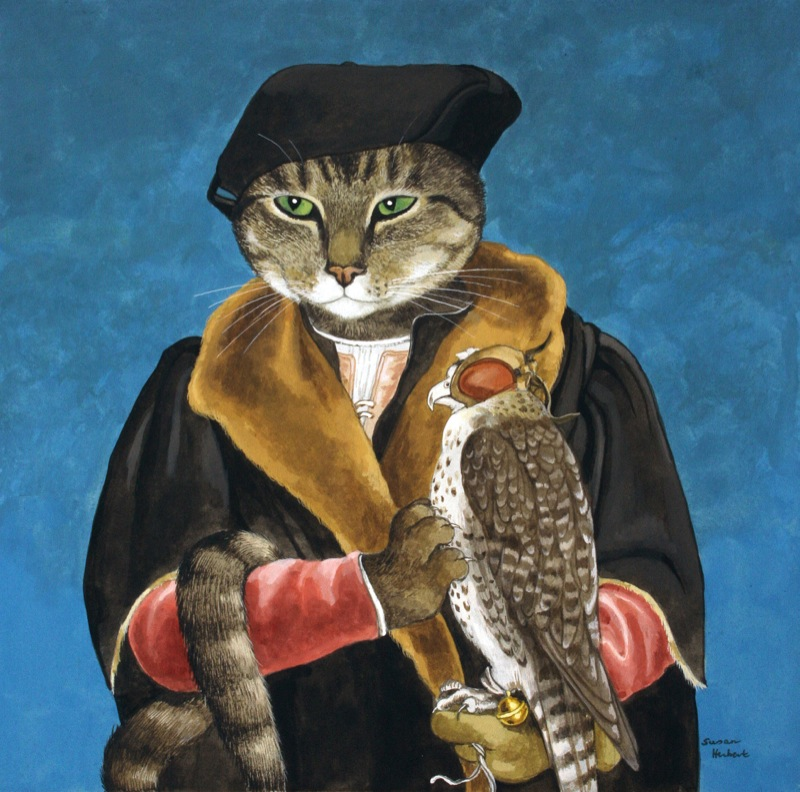
\includegraphics{cat-painting}
		\end{figure}
\end{document}
	\end{lstlisting}    
	
	\chapter{The Template} \label{chap:template}
	\section{Preamble} \label{sect:preamble}
	With these basics under our belt, we can decode the Lab Template. Let's look at the preamble together.	
	\begin{lstlisting}[numbers=left,xleftmargin=5mm]
%Template and commentary by Michael Rouleau: https://github.com/mikerouleau/ME4842.git
%Text primarily from Dr. Stutts' Systems Laboratory Manual
%Last Updated: Feb 17, 2019

%----This template includes equation captions and numbering BELOW the equation----%

\documentclass[11pt,letter]{report}
\usepackage[margin=1in]{geometry}
\usepackage[justification=centering, format=plain, font=it, margin=1in]{caption}
\usepackage{amsmath, amssymb}
\usepackage{graphicx}
\usepackage{float}
\usepackage{aliascnt}

\newaliascnt{eqfloat}{equation}
\newfloat{eqfloat}{!htb}{eqflts}
\floatname{eqfloat}{Equation}

\title{\Huge{Systems Lab \LaTeX\ Template Commentary}}
	\author{Section \#, Group \#: \\
		Group Member 1 \footnote{Missouri University of Science and Technology, Rolla, Missouri 65409} 
		\quad Group Member 2\footnotemark[1]
		\quad Group Member 3\footnotemark[1]
		\quad Group Member 4\footnotemark[1] 
		\\ GTA: Blaine Allen \\ \\ 
		Prepared By: \\ Michael Rouleau\footnote{Georgia Institute of Technology, Atlanta, Georgia 80813}
	}
\date{\today}
	\end{lstlisting}
	
	Lines 1-6 contain notes to whoever is reading the code. It is good practice to comment your name and date as a bare minimum, especially if someone may look at your source code later.
	
	Line 7 defines the document class, just like we did in Section \ref{sec:structure}. The only difference is now we have also specified values for a couple of options: paper size and normal text font size. While these may be set by a class, using an option overrides the default value.
	
	Lines 8-13 all include various external packages for increased customization. The geometry package allows us to define margins of 1". Caption changes the default font settings for our captions. Amsmath and amssymb provide some fancy commands and environments for math (note we're being sneaky and including two packages at once on this line). We'll primarily be using the equation environment. Graphicx allows us to insert figures with \verb|\includegraphics{imagefile}|. Finally, the float and aliascnt packages are used for some fancy manipulation of equations in order to meet the formatting requirements.
	
	Speaking of formatting gymnastics, lines 15-17 are where the most complex of it takes place. In line 15, we define a new alias count called ``eqfloat." This alias essentially acts as another name for the counter it follows, ``equation." This means if eqfloat is indexed, equation will be indexed and vice versa. Line 16 takes eqfloat and defines a float container also named ``eqfloat". [!htb] defines our preferred placements, and ``eqflts" is the name it uses for the log file. The float implicitly inherits the counter alias from line 16 - each eqnfloat environment is counted with the equation counter. Line 17 changes the name of the float to be ``Equation." By doing this, the \verb|\caption{A Clever Caption}| command will read \textit{Equation \#: A Clever Caption}, instead of \textit{eqfloat \#: A Clever Caption}.
	
	Finally lines 19-28 pertain to the title page. This section is fairly self-explanatory. However, you'll note the use of \verb|\quad| and \verb|\\| within the author command. \verb|\quad| helps with the spacing of authors. Even if you don't have 4 group members, \verb|\quad| will likely still work to distribute them in an aesthetic manner. \verb|\\|, on the other hand, serves as a complex macro that introduces a line break in this context. Limit the use of \verb|\\| unless necessary. Without adding additional packages, one way to add author affiliations is through the use of footnotes. The first author with a given affiliation gets the \verb|\footnote{My School}| command. Each following author gets \verb|\footnotemark[#]| to designate which affiliation they belong to. With this implementation, the affiliation number using \verb|\footnotemark[#]| does NOT auto-update. Be careful here. If you wish to explore a more flexible option, take a look at the authblk package.
	
	\section{Body} \label{sect:body struct}
	After the Preamble, \verb|\begin{document}| begins the document environment. Immediately after, we use the \verb|\maketitle| command to generate the title page of our document. Since the document body usage is repetitive, let's break up the template further into different environments and their usage.
	
	\newpage
	\subsection{Sections} \label{subsect: sections}
	Just as described in Section \ref{sect:org}, the command \verb|\section*{Section Title}| defines the beginning of a new section. The ``starred" version of this command removes the section number from showing up on your final report. For each new section, simply add the \verb|\section{}| command and type the name of the new section in curly brackets following it. Subsections may be nested within sections.
	
	\subsection{Tables} \label{subsect:table}
	Tables are perhaps the most difficult format to insert in \LaTeX{}. Fortunately, we can logically break down each line again.
	\begin{lstlisting}[numbers=left,xleftmargin=5mm]
	\begin{table}[!htb]
		\caption{Annual Per Capita Consumption of Mozzarella Cheese and Civil Engineering Doctorates Awarded \cite{Vigen}}
		\label{table:Civil Cheese}
		\centering
		\begin{tabular}{|c|c|c|}
			\hline
			\textbf{Year} & 
			\textbf{\begin{tabular}[c]{@{}c@{}}
				Civil Engineering\\ 
				Doctorates
			\end{tabular}} &
			\textbf{\begin{tabular}[c]{@{}c@{}}
				Mozzarella\\
				Cheese Consumption
			\end{tabular}} \\ \hline
			2000  & 480  & 9.3     \\ \hline
			2001  & 501  & 9.7     \\ \hline
			2002  & 540  & 9.7     \\ \hline
			2003  & 552  & 9.7     \\ \hline
			2004  & 547  & 9.9     \\ \hline
		\end{tabular}
	\end{table}
	\end{lstlisting}
	
	At this point, you should be able to guess what line 1 does - it marks the beginning of a table environment. Since tables are floating environments, the \verb|[!htb]| tag tells the compiler where to place the table, in order of preference. Refer to Section \ref{sect:org} for more options. Line 2 adds a caption for the table, complete with a citation - we'll get to those later, in Section \ref{sect:ref}. With this template, each table is automatically numbered as long as a caption exists
	Line 3 adds a reference label to the table. Again, we'll cover what this means in Section \ref{sect:ref}. Line 4 tells the compiler to center the current paragraph, or in this case, table.
	
	Line 5 is where the fun begins. First, we start a tabular environment within the table environment and define the number of columns (3) using \{$|$c$|$c$|$c$|$\}. Note that c does not refer to ''column." Instead, c refers to centered - the formatting for each column's data. Other popular options are ``l" for left and ``r" for right alignment. Line 6 inserts a horizontal line that is the width of our table. 
	
	Lines 7-15 start off easy - the first cell in our table, moving left to right from the top is Year, in bold text. \& signifies the end of the cell, and we move into our second cell on line 8. Picking this cell apart, we have a \verb|\textbf{}| command again - so this cell is also in bold text. Within it, another tabular environment starts. This second environment allows us to create subcells within the cell - one for ``Civil Engineering" and the other for ``Doctorates." Unfortunately, the standard tabular package does not support \verb|\newline| or \verb|\linebreak|, so this is the best native workaround I am aware of. In declaring this new tabular environment, we use \verb|[c]{@{}c@{}}| - different from the first time. \verb|[c]| in this case is our vertical alignment - again, centered. Other options include t for top and b for bottom. Our horizontal parameters are taken care of within the curly brackets. \verb|@{}| overrides any horizontal padding on each side of these subcells, and c is again horizontal alignment for the single column of subcells. The contents of each subcell is on lines 9 and 10, with a \verb|\\| to demarcate the end of a row. With an \$ to move us into the next cell, the same process is repeated for our final title cell. After all three cells in the top row are full, \verb|\\ \hline| is used to mark the end of the row and insert a horizontal line.
	
	Armed with this information, lines 16-22 should be easy to figure out. However, if you find tables confusing, you're in luck! For small data sets, there are several online tools to automatically generate \LaTeX{} tables. One such tool is located at \url{https://www.tablesgenerator.com/}. Some \LaTeX{} editors also include table-building functionality.
	
	\subsection{Figures} \label{subsect:fig}
	Figure insertion is a comparatively trivial process using the \verb|graphicx| package. Simply by looking at the code below, most of it should be easily understood.
	\begin{lstlisting}[numbers=left,xleftmargin=5mm]
\begin{figure}[!htb]
	\label{fig:Cat Lord}
	\centering
	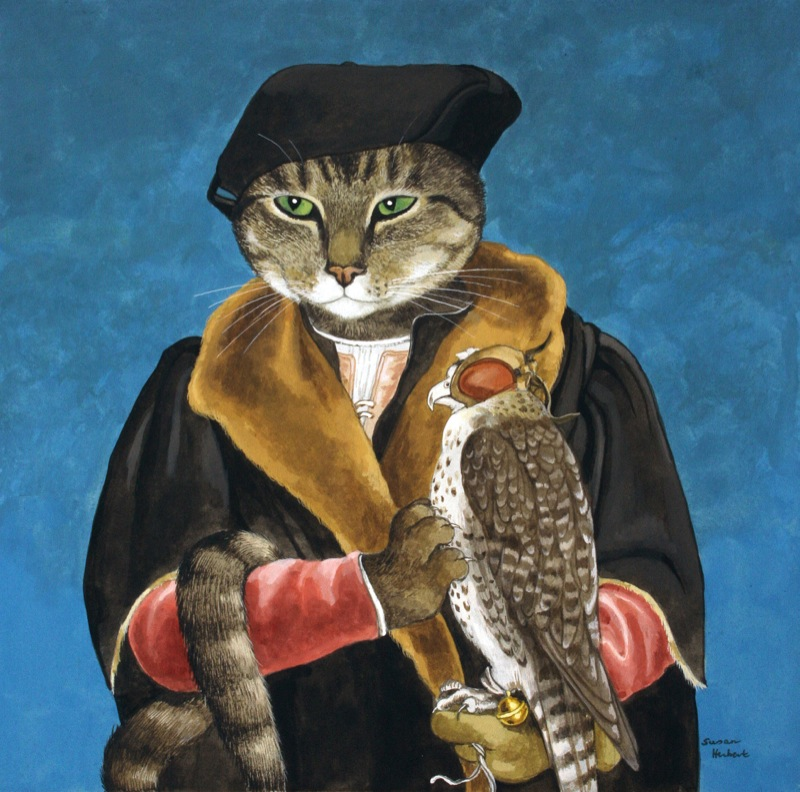
\includegraphics[scale=0.4]{cat-painting}
	\caption{Robert Cheseman (Holbein)\cite{Herbert}}
\end{figure}
	\end{lstlisting}
	
	As expected, \verb|\begin{figure}[!htb]| starts a figure environment. Figures are again floating environments, so we provide them with placement preferences. And as we've seen before, \verb|\label{key}| defines a label and \verb|\centering| centers the figure.
	
	The includegraphics command itself takes the form of  \verb|\includegraphics[options]{imagefile}|, where options are things like height, width, and scale. If you use an option such as height or width, be sure to include a unit (e.g. \verb|height=3cm|). Our feline friend is a bit on the large side, so we've scaled him down to 40\% of his original size. Purrfect! The imagefile field takes the filepath of the image as input - no need to add an extension, the compiler will search for all supported formats. Each time the compiler runs, it searches for the figure file and re-inserts it. This means that if you need to swap out a figure, simply upload the new figure to the same directory and rename the new and old files appropriately. Next time the compiler is run, the new figure will appear.
	
	Finally, we have a caption, complete with citation. With this template, each figure is automatically numbered as long as a caption exists - no need to keep track of figure numbers! For more information on citations, refer to Section \ref{sect:ref}.
	
	\pagebreak
	\subsection{Lists} \label{subsect:lists}
	A list is a convenient way to format the procedure section of a lab report. For most situations, a numbered list will suffice, taking the form of
	\begin{lstlisting}[numbers=left,xleftmargin=5mm]
\begin{enumerate}
	\item First item
	\item Second item
	\item Third item
\end{enumerate}
	\end{lstlisting}
	
	Here, we begin an enumerate environment and indicate the start of each line item as an \verb|\item|. The same process works for an unordered list using the \verb|itemize| environment. The syntax is identical.
	
	For more complex lists, it is possible to nest lists. For example, 
	\begin{lstlisting}[numbers=left,xleftmargin=5mm]
\begin{enumerate}
	\item First item
	\item \begin{enumerate}
		\item First subitem
		\item Second subitem
	\end{enumerate}
	\item \begin{itemize}
		\item First subitem
		\item Second subitem
	\end{itemize}
\end{enumerate}
	\end{lstlisting}
	
	generates the following list:
	
	\begin{enumerate}
		\item First item
		\item \begin{enumerate}
			\item First subitem
			\item Second subitem
		\end{enumerate}
		\item \begin{itemize}
			\item First subitem
			\item Second subitem
		\end{itemize}
	\end{enumerate}
	
	\subsection{Equations} \label{subsect:eqn}
	Equations are one of the significant strengths of any \LaTeX{} distribution. Instead of digging through symbol menus, complex functions can be typed quickly and intuitively.
	
	For short documents that require few equations, displaying equations inline with text may be appropriate. To enter math mode for this usage, enclose symbols in \$ signs (e.g. \$equation here\$).
	
	Alternatively, equations can be displayed separate from the main body of text by using the  \verb|eqfloat|  and  \verb|equation|  environments as shown in the following example. Note that these environments are nested to provide appropriate formatting with a label beneath the equation. The equation itself lies within the \verb|equation| environment. As before, the caption is specified with \verb|\caption{}|. A label is added to conveniently reference the equation elsewhere in the main text. When  in math mode, feel free to space equations out for code readability - almost all white space is ignored by the compiler.
	
	\begin{lstlisting}[numbers=left,xleftmargin=5mm]
\begin{eqfloat}
	\caption{The Quadratic Formula}
	\label{eq:quadratic}
	\begin{equation*}
		x_1 = \frac{-b \pm \sqrt{b^2 - 4ac}}{2a}
	\end{equation*}
\end{eqfloat}
	\end{lstlisting}
	
	The resulting equation appears as: 
	
	\begin{eqfloat}
		\caption{The Quadratic Formula}
		\label{eq:quadratic}
		\begin{equation*}
			x_1 = \frac{-b \pm \sqrt{b*2 - 4ac}}{2a}
		\end{equation*}
	\end{eqfloat}
	To label the equation using a right-justified number in parentheses, use the non-starred version of a \verb|\begin{equation}| environment. For instance, take the following code and its resulting form.
	\begin{lstlisting}
\begin{equation}
	\label{eq:Dirac}
	\left (
	\beta mc^2 + c 
	\left ( 
	\sum_{n=1}^3 \alpha_n p_n 
	\right )
	\right )
	\psi(x,t)
	=
	i \hbar \dfrac{\partial \psi(x,t) }{\partial t}
\end{equation}
	\end{lstlisting}

		\begin{equation}
	\label{eq:Dirac}
	\left (
	\beta mc^2 + c 
	\left ( 
	\sum_{n=1}^3 \alpha_n p_n 
	\right )
	\right )
	\psi(x,t)
	=
	i \hbar \dfrac{\partial \psi(x,t) }{\partial t}
		\end{equation}
	
	
	\section{References} \label{sect:ref}
	References can be hard to keep track of, especially with inline citations. \LaTeX{} helps keep track of your inline citations by using a reference key or label to specify a certain author, figure, or even section of the same document. As the document changes (e.g. you add a figure earlier in your report), the counter for the respective object changes (remember the counter we aliased for equations?). When this number changes, the number at each citation updates as well, keeping the entire document consistent. For example, take a figure given by
	
	\begin{lstlisting}[numbers=left,xleftmargin=5mm]
\begin{figure}[!htb]
	\label{fig:Cat Lord}
	\centering
	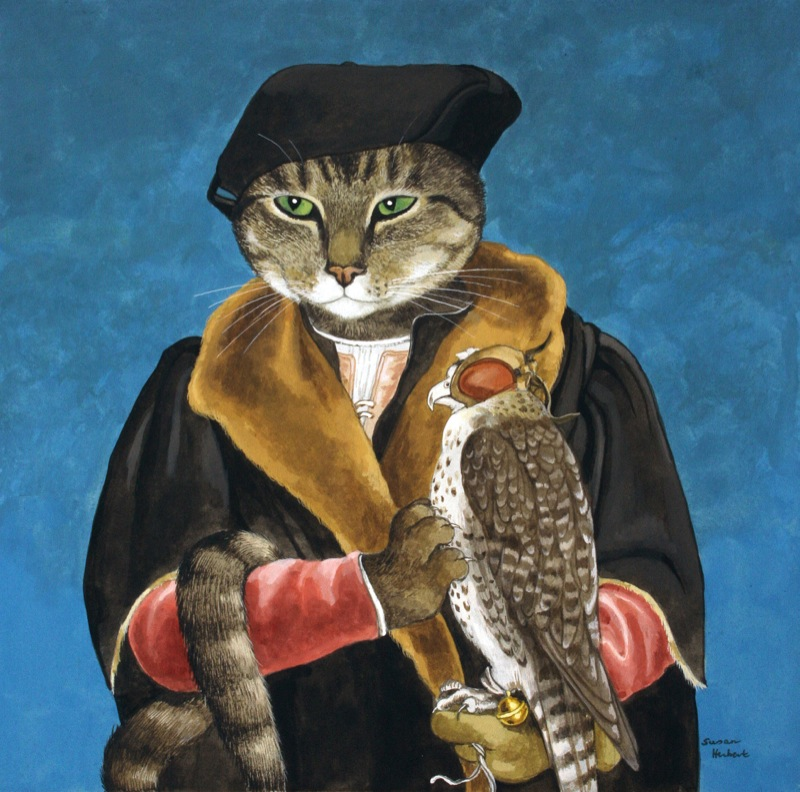
\includegraphics[scale=0.4]{cat-painting}
	\caption{Robert Cheseman (Holbein)\cite{Herbert}}
\end{figure}
	\end{lstlisting}
	
	Here, we've given Sir Cheseman the label ``Cat Lord." If I want to cite this figure elsewhere in my code, I would type ``\verb|Figure \ref{fig:Cat Lord}|" to refer to the painting, regardless of where it is in the document. For this figure, we also use the command \verb|\cite{key}|. Citations refer to the bibliography entries, which might look something like this for a pure \LaTeX{} document:
	
	\begin{lstlisting}[numbers=left,xleftmargin=5mm]
\begin{thebibliography}{9}

	\bibitem{Lamport}
	Lamport, L., \emph{LATEX: a document preparation system: users guide and reference manual.} Addison-wesley. 1994.
	
	\bibitem{Stutts}
	Stutts, D.S., \emph{Mechanical Engineering Systems Laboratory Manual.}
	Department of Mechanical and Aerospace Engineering, Missouri University of Science and Technology, 3 Oct. 2018. 130-131.
	
	\bibitem{Vigen}
	Vigen, T., \emph{15 Insane Things That Correlate With Each Other.}
	Spurious Correlations, tylervigen.com/spurious-correlations. Accessed 8 Nov. 2018.

\end{thebibliography}
	\end{lstlisting}
	
	The format here should look similar to a list, and with good reason - what is a bibliography but a list? On line one, we begin the bibliography environment and specify the number of references that are listed. For less than 10 references, the value 9 is commonly used, even if there are only 3 entries as in this case. For 10-99 entries, the value 99 is used.
	
	Each entry starts similar to the items in a list, but we use the \verb|\bibitem{key}\| command instead of \verb|\item|. The key argument is analogous to the label we use for equations and figures - this is how you cite the work elsewhere in the document. Just like using \verb|\ref{label}|, we use would cite Dr Stutts' bibliography number as \verb|\cite{Stutts}|.
	
	Complex projects can make use of an automatically generated bibliography, much like our front page. However, the methods to implement such a bibliography lies outside the scope of this document. I encourage interested readers to look up BibTeX reference management tools.
	
	\section{Including Code}
	For some experiments, it may be useful to include MATLAB code, especially in the appendix. While this template was not originally designed with that functionality, it can be easily modified to do so.
	
	The first step is to include the \verb|listings| package in the Preamble along with a couple options. To add a colored background for the code, also include \verb|xcolor|. Either way, brace yourself for all the options. It's easiest to just copy-paste the following code into your Preamble.
	
	\begin{lstlisting}
\usepackage{xcolor}
	\definecolor{lightgray}{gray}{0.93} %defines my custom gray
\usepackage{listings}
	\lstset{ 
		language=Matlab,
		numberstyle=\footnotesize,
		firstnumber=1,
		stepnumber=5,
		numberfirstline=true,
		breaklines=true,
		backgroundcolor=\color{lightgray},
		showspaces=false,
		showstringspaces=false,
		showtabs=false
	}
\renewcommand{\lstlistingname}{Code Snippet}
\renewcommand{\lstlistlistingname}{List of \lstlistingname s}
\end{lstlisting}

	Using this environment looks something like the following. Note that the label and caption syntax is different from the other environments we've looked at. We also define the file type here - it must be an m-code file. Live scripts (.mlx) will not properly import.

\begin{lstlisting}
\lstinputlisting[caption={Creative Caption}, label={mylabel}]{my_matlab_file.m}
\end{lstlisting}

	%A pure LaTeX bibliography 
	\begin{thebibliography}{3} %{3} is the number of entries to be added. The maximum value is 99.
		
		\bibitem{Herbert}
		Herbert, S.,\emph{Robert Cheseman (Holbein).}
		Chris Beetles Gallery, London, England, \url{www.chrisbeetles.com/gallery/animals/cats/robert-cheseman-holbein.html}. Accessed 8 Nov. 2018.
		
		\bibitem{Lamport}
		Lamport, L., \emph{LATEX: a document preparation system: user's guide and reference manual.} Addison-wesley. 1994.
		
		\bibitem{Overleaf}
		Overleaf c/o Digital Science., London, England, \url{https://www.overleaf.com/learn/latex/Positioning_of_Figures}. Accessed 16 Feb. 2019.
		
		\bibitem{Stutts}
		Stutts, D.S., \emph{Mechanical Engineering Systems Laboratory Manual.}
		Department of Mechanical and Aerospace Engineering, Missouri University of Science and Technology, 25 Jan. 2019. 142-146.
		
		\bibitem{Vigen}
		Vigen, T., \emph{15 Insane Things That Correlate With Each Other.}
		Spurious Correlations, tylervigen.com/spurious-correlations. Accessed 8 Nov. 2018.
		
		
		\bibitem{Gratzer}
		Gratzer, G.A., \emph{Practical LaTeX.} 2014.
		
	\end{thebibliography}
\end{document}